%%%%%%%%%%%%%%%%%%%%%%%%
% 3) Building EMTG in Visual Studio}
%%%%%%%%%%%%%%%%%%%%%%%%

Following the CMake configure-and-generate steps (Section~\ref{sec:setting_cmake_options}), open the project in Visual Studio. This can be done by clicking the ``Open Project'' button in the CMake \ac{GUI}. Then, perform the following actions:

\begin{enumerate}
	\item Right-click on ``EMTGv9'' in the Solution Explorer then click ``Set As Startup Project''.
		\begin{figure}[H]
			\centering
			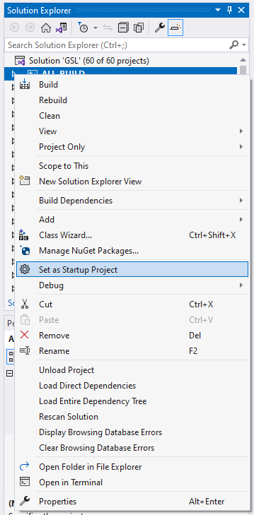
\includegraphics[width=0.35\linewidth]{../../../shared_latex_inputs/images/vstudio_set-startup.png}
			\caption{Visual Studio Select Startup Project}
		\end{figure}	
	\item In the toolbar, select the ``Release'' option from the ``Solution Configurations'' dropdown.
		\begin{figure}[H]
			\centering
			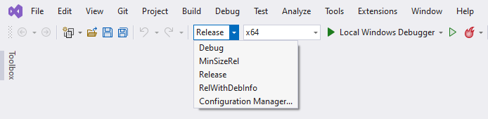
\includegraphics[width=0.7\linewidth]{../../../shared_latex_inputs/images/vstudio_config_release.png}
			\caption{Visual Studio Release Solution Configuration}
		\end{figure}
		\emph{Do not select ``Debug'' unless you actually want to debug \ac{EMTG}!}
	\item Right-click on ``EMTGv9'' in the Solution Explorer then click ``Build''.
	\item Verify the build is successful. \\ \emph{The log output will result in a message that says, in part, ``0 failed'' in the Visual Studio output window. In addition, Path/To/EMTG/Repo/bin will contain EMTGv9.exe and libsnopt.dll.}
\end{enumerate}